\documentclass[a4paper,12pt]{article}
\usepackage[utf8]{inputenc}
\usepackage[T2A]{fontenc}
\usepackage[russian]{babel}
\usepackage{amsmath, amssymb}
\usepackage{graphicx}
\usepackage{geometry}
\usepackage{listings}
\usepackage{makecell}
\usepackage{cancel}
\usepackage{ulem}
\usepackage{xcolor} % Для цветов
\usepackage{float}
\usepackage[colorlinks=true, linkcolor=blue, urlcolor=red, citecolor=green]{hyperref}
\usepackage{bm} % Для жирных математических символов
\newcommand{\diff}{\mathop{}\!\mathrm{d}} % Для правильного d в дифференциалах
\allowdisplaybreaks
\definecolor{backcolour}{rgb}{0.96,0.96,0.96} % Светлый фон
\definecolor{codegray}{rgb}{0.4,0.4,0.4}     % Серый для номеров строк
\definecolor{codepurple}{rgb}{0.58,0.44,0.86} % Светло-фиолетовый для строк
\definecolor{commentgreen}{rgb}{0.22,0.55,0.33} % Зелёный для комментариев
\definecolor{keywordblue}{rgb}{0.25,0.5,0.75} % Насыщенный синий для ключевых слов
\definecolor{identifierorange}{rgb}{0.85,0.4,0.12} % Тёплый оранжевый для переменных
\definecolor{functionyellow}{rgb}{0.88,0.73,0.38} % Песочный жёлтый для функций
\definecolor{numberred}{rgb}{0.8,0.2,0.2}    % Красный для чисел

\lstset{
    language=Python,
    columns=fullflexible,
    backgroundcolor=\color{backcolour},
    commentstyle=\color{commentgreen},
    keywordstyle=\color{keywordblue},
    identifierstyle=\color{identifierorange},
    numberstyle=\tiny\color{codegray},
    stringstyle=\color{codepurple},
    basicstyle=\ttfamily\small,
    breaklines=true,
    frame=single,
    tabsize=2,
    showstringspaces=false,
}
\geometry{top=1.2cm, bottom=1.2cm, left=1.2cm, right=1.2cm}

\title{Курсовая работа.}
\author{Козлов Кирилл 305 группа}
\date{\today}

\begin{document}



\thispagestyle{empty}
\begin{center}
\textbf{Федеральное государственное бюджетное\\
образовательное учреждение высшего образования\\
«Московский государственный университет имени М. В. Ломоносова»}

\vspace{0.5em}
\textit{Факультет Вычислительной математики и кибернетики \\}
\textit{Кафедра вычислительных методов}

\vspace{3em}
Козлов Кирилл Андреевич

\vspace{2em}
\textbf{\LARGE "Численные методы решения динамических задач, возникающих в детерминированных моделях экономического равновесия"}

\vspace{2em}
Курсовая работа\\
по направлению подготовки:\\ 
01.03.02 «Прикладная математики и информатика»\\
\end{center}

\vspace{25em}
\begin{tabular}{p{5cm}p{5cm}p{5cm}}
     & & Научный руководитель: \\
     & & д. ф.-м, профессор \\
    \noalign{\vspace{3em}}
     & & \underline{\hspace{5cm}} \\
     & & С.\,В.~Богомолов \\
\end{tabular}

\vfill
\begin{center}
Москва, 2025
\end{center}
\newpage

\tableofcontents

\newpage







\section{Введение}
{\fontsize{14pt}{20pt}\selectfont 
\hspace{1em}Математические модели играют ключевую роль в экономике, позволяя формализовать сложные процессы, прогнозировать развитие систем и находить оптимальные управленческие решения. Особое значение имеют задачи оптимального управления, возникающие в экономических моделях, поскольку они помогают определить наилучшие стратегии распределения ресурсов, инвестирования и управления капиталом.

Численные методы решения таких задач активно развиваются, однако их эффективность может существенно различаться в зависимости от типа модели и условий. Сопоставление различных подходов позволяет выявить наиболее подходящие методы для конкретных экономических приложений. На данном этапе исследования рассматриваются детерминированные модели, что упрощает анализ и позволяет сосредоточиться на сравнительных характеристиках численных алгоритмов.

\subsection{Цель работы}
\hspace{1em}Целью курсовой работы является анализ и сравнение численных методов решения задач оптимального управления, возникающих в экономических моделях.

\subsection{Задачи исследования}
\begin{itemize}
    \item Рассмотреть основные математические модели в экономике, приводящие к задачам оптимального управления.

    \item Изучить классические и современные численные методы решения таких задач.

    \item Провести сравнительный анализ эффективности методов на примере конкретных экономических моделей.

    \item Сделать выводы о применимости рассмотренных подходов в детерминированном случае.
\end{itemize}
\subsection{Структура работы}
Курсовая работа состоит из введения, нескольких глав, заключения и списка литературы. В первой главе рассматриваются теоретические основы математических моделей в экономике и задачи оптимального управления. Во второй главе анализируются численные методы их решения. В третьей главе проводится сравнительное моделирование и обсуждаются результаты.

Таким образом, данное исследование направлено на систематизацию подходов к решению экономических задач оптимального управления и оценку эффективности численных методов в детерминированном случае.

}



\section{Описание RBC-модели(Real Business Cycle model, модель реального делового цикла)}
{\fontsize{14pt}{20pt}\selectfont Рассмотрим детерминированный вариант модели реального делового цикла
Классическая RBC-модель описывается двумя задачами для домохозяйств и фирм, условиями равновесия на тех рынках (товаров, капитала и труда) и замыкается балансовыми макроэкономическими тождествами. Единственным активом в экономике является производственный капитал, а его собственником являются домохозяйства. Цены на товарном рынке в модели нормированы к единице и все колическивенные величины измеряются в единицах товаров и услуг потребления (это можно считать шкалой относительных цен).
Агенты в модели (домохозяйства и фирмы) репрезентативные, а все рынки являются совершенно конкурентными. В условиях совершенной конкуренции на эквивалентным вариантом будет модель с социальным планировщиком (сослаться на 1ю теорему Благосотояния и на теорему Эрроу-Дербе).

\subsection{Построение модели}
\subsubsection{Задача домохозяйства}
Домохозяйство максимизирует ожидаемый ($E_0$) функционал полезности $U$ \eqref{eq:formula_1}, представляющий собой бесконечную сумму дисконтированных мгновенных полезностей (с дисконтом $\beta$). Мгновенная полезность $u[\cdot]$ положительно зависит от потребления $C_t$ в периоде $t$ и отрицательно от количества трудозатрат $L_t$ в периоде $t$:
\begin{equation}
U = \max_{C, \, L} E_0 \sum_{t=0}^{\infty} \beta^t u[C_t, \, L_t] \, , \quad 0 < \beta < 1 
\label{eq:formula_1}
\end{equation}

При соблюдении балансового ограничения \eqref{eq:formula_2} и с учетом правила накопления активов \eqref{eq:formula_3}:

\begin{equation}
C_t + I_t = W_t L_t + R_t K_t \quad ,
\label{eq:formula_2}
\end{equation}

\begin{equation}
K_{t+1} = (1 - \delta) K_t + I_t \quad ,
\label{eq:formula_3}
\end{equation}

где $K_t$ -- объем капитала (активов), $I_t$ -- инвестиции, $W_t$ -- зарплата, $R_t$ -- процентная ставка по активам, которые домохозяйства сдают в аренду фирмам, $\delta$ -- коэффициент амортизации (устаревания капитала). В этой простой постановке эти два условия можно объединить \eqref{eq:formula_4}:

\begin{equation}
K_{t+1} = (1 - \delta) K_t + W_t L_t + R_t K_t - C_t \quad .
\label{eq:formula_4}
\end{equation}

\subsubsection{Задача фирмы}

Фирма максимизирует прибыль в каждом периоде, выбирая оптимальный объем капитала и труда, т.е. решает задачу \eqref{eq:formula_5}:

\begin{equation}
Profit = \max_{K, L} \left\{ A e^{z_t} F(K_t, L_t) - W_t L_t - R_t K_t \right\}
\label{eq:formula_5}
\end{equation}

где $F(K_t, L_t) = Y_t$ -- производственная функция, $A$ -- уровень технического прогресса, $z_t$ -- совокупная факторная производительность (СФП), которая описывается следующим AR(1)-процессом \eqref{eq:formula_6}:

\begin{equation}
z_t = \mu z_{t-1} + \varepsilon_t, \quad \varepsilon_t \sim N(0, \sigma_z^2), \quad 0 \leq \mu < 1
\label{eq:formula_6}
\end{equation}

где $\mu$ -- коэффициент персистентности, $\varepsilon_t$ -- шок, $\sigma_z^2$ -- дисперсия шока СФП.

Замыкающее макроэкономическое тождество имеет вид \eqref{eq:formula_7}:

\begin{equation}
C_t + I_t = A e^{z_t} F(K_t, L_t)
\label{eq:formula_7}
\end{equation}

Условия равновесия состоят в равенстве спроса и предложения на всех рынках \eqref{eq:formula_8}:

\begin{equation}
Y_t^{demand} = Y_t^{supply}, \quad L_t^{demand} = L_t^{supply}, \quad K_t^{demand} = K_t^{supply}
\label{eq:formula_8}
\end{equation}

Эти функции спроса и предложения от соответствующих цен $(1, W_t, R_t)$ выводятся благодаря получению необходимых условий для задачи домохозяйства и задачи фирмы.


\subsubsection{Необходимые условия экстремума (F.O.C.) - для домохозяйства}
Возьмём функцию полезности:
\[
    u = ln(C_t(i)) - \varphi \frac{L_t(i)^{1+\psi}}{1 + \psi}
\]

\smallskip
\noindent{где есть две константы:}
\begin{itemize}
    \item $\psi$ -- величина, обратная к эластичности труда по Фришу
    \item $\varphi$ -- фактор ненависти к труду
\end{itemize}

Составим функцию Лагранжа для уравнения \eqref{eq:formula_1} и ограничений \eqref{eq:formula_4}:
\begin{align*}
\mathcal{L} &= \sum_{t=0}^{\infty} \beta^t \left[ \ln C_t(i)  - \varphi \cdot \frac{L_t(i)^{1+\psi}}{1 + \psi} \right] + \\ 
    &\quad + \sum_{t=0}^{\infty} \lambda_{1,t} \left( W_t L_t + R_t K_t - C_t - I_t \right) 
    + \sum_{t=0}^{\infty} \lambda_{2,t} \left( (1-\delta) K_t + T_t - K_{t+1} \right) \rightarrow \max_{C, I, K, \lambda} 
\end{align*}

Если применим F.O.C. к функции Лагранжа то получим 4 уравнения уравнения:
\begin{align*}
    \text{1) } & \mathcal{L^{'}_{C}} = \beta^{t} \cdot \frac{1}{C_t(i)} - \lambda_{1,t} \quad  \equiv 0  \\
    \text{2) } & \mathcal{L^{'}_{L}}= -\beta^{t} \cdot \varphi \cdot L_t(i)^{\psi} + \lambda_{1,t} \cdot W_t \quad  \equiv 0  \\
    \text{3) } & \mathcal{L^{'}_{I}}= -\lambda_{1,t} + \lambda_{2,t} \quad   \equiv 0\\
    \text{4) } & \mathcal{L^{'}_{K}}= -\lambda_{2,t} + \lambda_{2,t+1} (1-\delta) + \lambda_{1,t+1} \cdot R_{t+1} \quad  \equiv 0  
\end{align*}

Из первого и третьего уравнения выводим:
\begin{align*}
    \lambda_{1,t} &= \frac{\beta^{t}}{C_t(i)}    \\
    \lambda_{1,t} &= \lambda_{2,t}
\end{align*}

Так как  $ \lambda_{1,t} = \lambda_{2,t}$ ,то из первого и второго уравнения можно выразить условие оптимальности труда:
\begin{align*}
    \lambda_{1,t} = \frac{\beta^{t}}{C_t(i)} \\
    \lambda_{1,t} = \frac{\beta^{t} \varphi L^{\psi}}{W_{it}} \\
    \frac{1}{C_{t}(i)} = \frac{\varphi L_{it}^\psi}{W_{it}}
\end{align*}
Преобразуем четвертое уравнение, подставив $\lambda_{1,t} = \lambda_{2,t}$:
\begin{align*}
    -\lambda_{1,t} + \lambda_{1,t+1}(1-\delta) + \lambda_{1,t+1}R_{t+1} = 0  \\
    \lambda_{1,t+1}(1+R_{t+1}-\delta) = \lambda_{1,t}  \\
    \frac{\lambda_{1,t+1}}{\lambda_{1,t}}(1+R_{t+1}-\delta)  = 1 \\ 
\end{align*}
Так как $\lambda_{1,t} = \frac{\beta^{t}}{C_t(i)}$ , то это уравнение можно переписать:
\[
    \beta(1+R_{t+1}-\delta)  = \frac{C_{t+1}}{C_{t}}
\]
Это уравнение называется уравнением Эйлера.



\subsubsection{Необходимые условия экстремума (F.O.C.) - для фирмы}
Поскольку мы рассматриваем рынки с совершенной конкуренцией, то можно переписать производственную функцию $F(K_t, L_t) = Y_t$ , как 
\[ 
    F(K_t, L_t) = K^{\alpha}_{t}L^{1-\alpha}_{t}
\] 
где $\alpha$ - факторная эластичность капитала.
Также поскольку в совершенной конкуренции у фирм отсутствует прибыль и весь продукт должен распределяться между собственниками капитала и труда, то можно утверждать ,что $Ae^{z_{t}}F(K_t, L_t) = W_{t}L_{t} + R_{t}K_{t}$

Применим F.O.C. , получим:
\begin{align*}
    \text{1) } & F^{'}_{k} = R_{t} \quad \Rightarrow \alpha K^{\alpha-1}_{t}L^{1-\alpha}_{t} = R_{t} \\
    \text{2) } & F^{'}_{L} =  W_t \quad  \Rightarrow (1-\alpha)K^{\alpha}_{t}L^{-\alpha}_{t} = W_t   \\
\end{align*}
Отсюда можнем выразить зарплату и процентную ставку на капитал:
\begin{align}
    R_t &= \alpha \frac{Y_t}{K_t} \label{eq:capital_share} \\
    W_t &= (1-\alpha) \frac{Y_t}{L_t} \label{eq:labor_share}
\end{align}

\subsubsection{Итоговая система}
Итого получим систему из 7 уравнений:
\begin{equation}
    \begin{cases}
    \begin{alignedat}{2}
    &\text{Уравнение Эйлера:} 
    && \beta (1 + R_{t+1} - \delta) = \frac{C_{t+1}}{C_t} \\
    &\text{Оптимальность труда:} 
    && \frac{1}{C_t(i)} = \frac{\varphi L_{it}^\psi}{W_{it}} \\
    &\text{Доходность капитала:} 
    && R_t = \alpha \frac{Y_t}{K_t} \\
    &\text{Заработная плата:} 
    && W_t = (1-\alpha) \frac{Y_t}{L_t} \\
    &\text{Ресурсное ограничение:} 
    && Y_t = C_t + I_t \\
    &\text{Накопление капитала:}
    && K_{t+1} = I_t + (1-\delta)K_t \\
    &\text{Производственная функция(Кобб-Дуглас): }
    && Y_t = K_t^\alpha L_t^{1-\alpha} \\
    &\text{Распределение дохода:}
    && F(K_t,L_t) = W_t L_t + R_t K_t = Y_t \\
    \end{alignedat}
    \end{cases}
    \label{eq:system}
\end{equation}

Нужно найти общее равновесие системы - равновесие на всех рынках.Для этого сначала найдём стационарное состояние:
\begin{align}
    C_t &= C_{t+1} = C^{*}  \\
    K_t &= K_{t+1} = K^{*}
\end{align}

Получим следующее:
\begin{equation}
    \begin{cases}
    \begin{alignedat}{2}
    R^{*} &= (\frac{1}{\beta} - 1 + \delta) \\
    L^{*} &= \left(\frac{W^{*}}{\varphi C^{*}}\right)^{\frac{1}{\psi}}\\
    R^{*} &= \alpha \frac{Y^{*}}{K^{*}} \\
    W^{*} &= (1-\alpha) \frac{Y^{*}}{L^{*}} \\
    Y^{*} &= C^{*} + I^{*} \\
    I^{*} &= \delta K^{*} \\
    Y^{*} &= K^{* \alpha} L^{* (1-\alpha)}
    \end{alignedat}
    \end{cases}
    \label{eq:system_stationary}
\end{equation}

\noindent\textbf{Параметры модели:}
\begin{align*}
    \alpha &\in (0,1)    &&\text{-- факторная эластичность капитала} \\
    \beta  &\in (0,1)   &&\text{-- коэффициент дисконтирования} \\
    \delta &\in [0,1]   &&\text{-- коэффициент амортизации (устаревания капитала)} \\
    \psi    &> 0      &&\text{-- величина, обратная к эластичности труда по Фришу} \\
    \varphi &> 0      &&\text{-- фактор ненависти к труду}
\end{align*}

\subsubsection{Поиск стационарной точки}
Дана следующая система уравнений:
\begin{align}
    R^* &= \frac{1}{\beta} - 1 + \delta, \label{eq1} \\
    L^* &= \left( \frac{W^*}{\varphi C^*} \right)^{\frac{1}{\psi}}, \label{eq2} \\
    R^* &= \alpha \frac{Y^*}{K^*}, \label{eq3} \\
    W^* &= (1-\alpha) \frac{Y^*}{L^*}, \label{eq4} \\
    Y^* &= C^* + I^*, \label{eq5} \\
    I^* &= \delta K^*, \label{eq6} \\
    Y^* &= K^{* \alpha} L^{* (1-\alpha)}. \label{eq7}
\end{align}

В (\ref{eq3}) подставим (\ref{eq7}):
\begin{equation*}
    R^* = \alpha K^{*(\alpha - 1)} L^{*(1- \alpha)} = \alpha \left(\frac{K^*}{L^*} \right)^{\alpha - 1} 
\end{equation*}

Тогда 
\begin{equation*}
    \left(\frac{R^*}{\alpha}\right)^{\frac{1}{\alpha - 1}} = \frac{K^*}{L^*}  
\end{equation*}

В (\ref{eq4}) подставим (\ref{eq7}):
\begin{equation*}
    W^* = (1-\alpha) \frac{Y^*}{L^*} = (1-\alpha) K^{*\alpha}L^{*-\alpha} = (1-\alpha)\left(\frac{K^*}{L^*}\right)^{\alpha} 
\end{equation*}

Тогда 
\begin{equation*}
    W^* = (1-\alpha) \left(\frac{R^*}{\alpha}\right)^{\frac{\alpha}{\alpha - 1}}
\end{equation*}

Преобразуем $Y^*$
\begin{equation*}
    Y^* = K^{* \alpha}L^{*(1-\alpha)} = L^* \left( \frac{K^*}{L^*}\right)^{\alpha} = L^* \left( \frac{R^*}{\alpha}\right)^{\frac{\alpha}{\alpha - 1}}
\end{equation*}
Преобразуем $K^*$ из (\ref{eq3})
\begin{equation*}
    K^* = \alpha \frac{Y^*}{R^*} = \alpha \frac{L^* \left( \frac{R^*}{\alpha}\right)^{\frac{\alpha}{\alpha - 1}}}{R^*}
\end{equation*}
Подставим в (\ref{eq5}) $Y^*$, $K^*$ и (\ref{eq6})
\begin{align*}
    L^* \left( \frac{R^*}{\alpha}\right)^{\frac{\alpha}{\alpha - 1}} = C^* + \delta K^* \\
    L^* \left( \frac{R^*}{\alpha}\right)^{\frac{\alpha}{\alpha - 1}} - \delta \alpha \frac{L^* \left( \frac{R^*}{\alpha}\right)^{\frac{\alpha}{\alpha - 1}}}{R^*} - C^* = 0 \\
    L^* \left( \frac{R^*}{\alpha}\right)^{\frac{\alpha}{\alpha - 1}} \left(1 - \frac{\delta \alpha}{R^*} \right) - C^* = 0
\end{align*}
\subsubsection{Итоговые выражения}
Оптимальные значения труда и потребления выражается через систему:
\begin{equation}
    \begin{cases}
    \begin{alignedat}{2}
    R^* &= \frac{1}{\beta} - 1 + \delta, \\
    L^* &\left( \frac{R^*}{\alpha}\right)^{\frac{\alpha}{\alpha - 1}} \left(1 - \frac{\delta \alpha}{R^*} \right) - C^* = 0, \\
    L^* &= \left( \frac{W^*}{\varphi C^*} \right)^{\frac{1}{\psi}},  \\
    K^* &= \alpha \frac{L^* \left( \frac{R^*}{\alpha}\right)^{\frac{\alpha}{\alpha - 1}}}{R^*}
    \end{alignedat}
    \end{cases}
    \label{eq:system_stationary_2}
\end{equation}
Решение этой системы можно найти методом Ньютона или методом деления отрезка пополам.
\subsubsection{Лог-линеаризация}
Нам нужно линеаризовать два уравнения:
\begin{equation}
    \begin{cases}
    \begin{alignedat}{2}
    K_{t+1} &= F(K_t,L_t) + (1 - \delta)K_t - C_t, \\
    1 &= \frac{C_t}{C_{t+1}} \beta \left( 1 + F^{'}_{K_t}(K_t,L_t) - \delta\right), \\
    \end{alignedat}
    \end{cases}
    \label{eq:system_dynamic}
\end{equation}
Делаем подстановки:
\[x_t = x^* \left( 1 + \frac{x_t - x^*}{x^*} \right) = x^*(1 + \tilde{x})\]

\[x_t = x^* \left( 1 + \ln \left( \frac{x_t}{x^*} \right) \right) = x^*(1 + \hat{x}) = x^* \left( 1 + \ln \left( 1 + \frac{x_t - x^*}{x^*} \right) \right) \approx x^*(1 + \tilde{x})\]

\[e^{x_t} \approx (1 + x_t)\]
Производственная функция:
\[
K_{t}^{\alpha} = \left[ K^{*} e^{\ln\left( \frac{K_{t}}{K^{*}} \right)} \right]^{\alpha} 
= K^{*\alpha} e^{\alpha \ln\left( \frac{K_{t}}{K^{*}} \right)} 
\approx K^{*\alpha} \left( 1 + \alpha \ln\left( 1 + \frac{K_{t} - K^{*}}{K^{*}} \right) \right) 
\approx K^{*\alpha} (1 + \alpha \widetilde{K}_{t})
\]


Уравнение Эйлера лог-линеаризуем сразу для более сложного случая функции полезности \( u(c_t) = \frac{c_t^{1-\sigma}-1}{1-\sigma} \):

\[
\begin{aligned}
\left( \frac{C_{t+1}}{C_t} \right)^{-\sigma} 
&= \left( \frac{C^* e^{\ln(C_{t+1}/C^*)}}{C^* e^{\ln(C_t/C^*)}} \right)^{-\sigma} \\
&= \left( \frac{C^*}{C^*} \right)^{-\sigma} \left( e^{\ln(c_{t+1}/C^*) - \ln(C_t/C^*)} \right)^{-\sigma} \\
&= e^{-\sigma \left[ \ln(C_{t+1}/C^*) - \ln(C_t/C^*) \right]} \\
&\approx 1 - \sigma \left( \ln\left(\frac{C_{t+1}}{C^*}\right) - \ln\left(\frac{C_t}{C^*}\right) \right) \\
&\approx 1 - \sigma (\hat{C}_{t+1} - \hat{C}_t)
\end{aligned}
\]

Собираем все вместе и получаем систему:

\begin{equation}
    \begin{cases}
    \begin{alignedat}{2}
    \beta \left[ 1 - \sigma (\tilde{C}_{t+1} - \tilde{C}_t) \right] \left[ \alpha A K^{*-\alpha-1} \left( 1 + (\alpha - 1)\tilde{K}_{t+1} \right) + 1 - \delta \right] &= 1 \\
    K^*(1 + \tilde{K}_{t+1}) = A K^{*-\alpha} (1 + \alpha \tilde{K}_t) + (1 - \delta) K^*(1 + \tilde{K}_t) - C^*(1 + \tilde{C}_t)
    \end{alignedat}
    \end{cases}
    \label{eq:system_dynamic_2}
\end{equation}

Упростим, избавляясь от «нулевого порядка» и учитывая, что \( A\alpha(K^*)^{\alpha-1} + 1 - \delta = 1/\beta \):

\[
\begin{aligned}
\beta \left[1 - \sigma (\hat{C}_{t+1} - \hat{C}_t)\right] \left[ \frac{1}{\beta} + \alpha (\alpha - 1) A K^{*-\alpha-1} \tilde{K}_{t+1} \right] &= 1 \\
\left[1 - \sigma (\hat{C}_{t+1} - \hat{C}_t)\right] \left[1 + \beta \alpha (\alpha - 1) A K^{*-\alpha-1} \tilde{K}_{t+1}\right] &= 1
\end{aligned}
\]

После раскрытия скобок и отбрасывания членов более высокого порядка (по Тейлору):
\[
1 - \sigma (\hat{C}_{t+1} - \hat{C}_t) + \beta \alpha (\alpha - 1) A K^{*-\alpha-1} \tilde{K}_{t+1} = 1
\]

Упрощенное уравнение:
\[
\sigma (\hat{C}_{t+1} - \hat{C}_t) = \beta \alpha (\alpha - 1) A K^{*-\alpha-1} \tilde{K}_{t+1}
\]

Получим следующую систему уравнений:

\begin{equation}
    \begin{cases}
    \begin{alignedat}{2}
    \sigma \tilde{C}_{t+1} - \beta \alpha (\alpha - 1) K^{* \alpha - 1} \tilde{K}_{t+1} = \sigma \tilde{C}_t \\
    \tilde{K}_{t+1} = \frac{1}{\beta} \tilde{K}_t - \frac{C^*}{K^*} \tilde{C}_t
    \end{alignedat}
    \end{cases}
    \label{eq:system_dynamic_3}
\end{equation}


В матричном виде эта система имеет следующий вид:

\[
\begin{pmatrix}
1 & -\beta \alpha (1-\alpha) K^{*\alpha-1} \\
0 & \sigma
\end{pmatrix}
\begin{pmatrix}
\tilde{K}_{t+1} \\
\tilde{C}_{t+1}
\end{pmatrix}
=
\begin{pmatrix}
\frac{1}{\beta} & -\frac{C^*}{K^*} \\
0 & \sigma
\end{pmatrix}
\begin{pmatrix}
\tilde{K}_t \\
\tilde{C}_t
\end{pmatrix}
\]

%Эту систему надо решить – например, методом Бланшара-Кана (о нем позднее). Перепишем эту систему как:
Перепишем эту систему как:
\[
\begin{pmatrix}
\tilde{K}_{t+1} \\
\tilde{C}_{t+1}
\end{pmatrix}
= B^{-1}D
\begin{pmatrix}
\tilde{K}_t \\
\tilde{C}_t
\end{pmatrix}
= A
\begin{pmatrix}
\tilde{K}_t \\
\tilde{C}_t
\end{pmatrix}
\]

где:
\begin{itemize}
\item $B = \begin{pmatrix}
1 & -\beta \alpha (1-\alpha) K^{*\alpha-1} \\
0 & \sigma
\end{pmatrix}$ 
\item $D = \begin{pmatrix}
\frac{1}{\beta} & -\frac{C^*}{K^*} \\
0 & \sigma
\end{pmatrix}$ 
\item $A = B^{-1}D$
\end{itemize}


Эту матрицу можем факторизовать классическим образом: $A = Q \Lambda Q^{-1}$. Тогда получим:

\[
\begin{pmatrix}
\tilde{K}_{t+1} \\
\tilde{C}_{t+1}
\end{pmatrix} 
= Q \Lambda Q^{-1} 
\begin{pmatrix}
\tilde{K}_t \\
\tilde{C}_t
\end{pmatrix}, 
\quad \text{где } 
\Lambda = \begin{pmatrix}
\lambda_1 & 0 \\
0 & \lambda_2
\end{pmatrix}
\]

Перейдём к системе в новых координатах с центром в нуле:

\[
Q^{-1} \begin{pmatrix}
\tilde{K}_{t+1} \\
\tilde{C}_{t+1}
\end{pmatrix} 
= \Lambda Q^{-1} \begin{pmatrix}
\tilde{K}_t \\
\tilde{C}_t
\end{pmatrix}
\]

Введём новые переменные:

\[
\begin{pmatrix}
y_{1,t} \\
y_{2,t}
\end{pmatrix} 
= Q^{-1} \begin{pmatrix}
\tilde{K}_t \\
\tilde{C}_t
\end{pmatrix} 
\quad \text{или явно:}
\quad 
\begin{cases}
y_{1,t} = q_{11} \tilde{K}_t + q_{12} \tilde{C}_t \\
y_{2,t} = q_{21} \tilde{K}_t + q_{22} \tilde{C}_t
\end{cases}
\]

Тогда система принимает диагональный вид:

\[
\begin{pmatrix}
y_{1,t+1} \\
y_{2,t+1}
\end{pmatrix} 
= \Lambda \begin{pmatrix}
y_{1,t} \\
y_{2,t}
\end{pmatrix} 
\quad (*)
\]

Для экономических задач чаще всего получаем, что $0 < \lambda_1 < 1 < \lambda_2$:
\begin{itemize}
    \item Сепаратриса, соответствующая $\lambda_1$, ведёт к нулю (устойчивое направление)
    \item Сепаратриса, соответствующая $\lambda_2$, уводит от нуля (неустойчивое направление)
\end{itemize}

\subsection{Построение оптимального правила для потребления}
Оптимальное правило $C_t = g(K_t)$ следует выбрать так, чтобы в системе (*) выполнялось $y_{2,t} = y_{2,t+1} = 0$. Это даёт:
\[
y_{2,t} = \tilde{q}_{21}\tilde{K}_t + \tilde{q}_{22}\tilde{C}_t = 0
\]
\[
\tilde{C}_t = \frac{\tilde{q}_{21}}{\tilde{q}_{22}}\tilde{K}_t = \tilde{q}\tilde{K}_t
\]
где $\tilde{q} \equiv \tilde{q}_{21}/\tilde{q}_{22}$ - ключевой параметр.

\subsection{Модель в пространстве состояний}
С учётом уравнения накопления капитала:
\[
\tilde{K}_{t+1} = \frac{1}{\beta}\tilde{K}_t - \frac{C^*}{K^*}\tilde{C}_t
\]
получаем замкнутую систему:
\begin{align*}
\text{Правило потребления (state equation)} &: \tilde{C}_t = \tilde{q}\tilde{K}_t \\
\text{Уравнение перехода (transition equation)} &: \tilde{K}_{t+1} = \left( \frac{1}{\beta} - \frac{C^*}{K^*}\tilde{q} \right)\tilde{K}_t
\end{align*}
С этой системой уже можно работать статистически: оценивать коэффициенты так, чтобы динамика модели была близка
фактической динамике наблюдаемых переменных.

\section{Уравнение Бэллмана}

Функция Бэллмана имеет следующий вид:
\[
    B(y_{\tau}, \tau) = \max_{(y,u) \in D} \left[ \int_{\tau}^{T} \varphi(u, y, t) dt + \psi (y(T)) \right]
\]

Принцип оптимальности по Беллману: оптимальная траектория управления $u$, выбираемые для отрезка $[\tau, \tau + \Delta \tau]$ должны быть такими, чтобы максимизировать вклад отрезка в критерий в сумме с критериями на оставшейся части времени.
\begin{align}
    B(y_{\tau}, \tau) &= \max_{(y,u)^{\tau + \Delta \tau}_{\tau}} \left[ \int_{\tau}^{\tau + \Delta\tau} \varphi(y, u, t) dt + B(y + \Delta y, \tau + \Delta\tau) \right] \label{eq:bellman} \\
    \dot{y} &= f(y, u, t) ,\quad  y(\tau) = y_{\tau} \label{eq:dynamics} \\
    \Delta y &= y(\tau + \Delta\tau) - y(\tau) \label{eq:delta_y} \\
    u(t) &\in \mathcal{U}(t) \label{eq:control_set} 
\end{align}

\subsection{Вывод уравнения Бэллмана}
\begin{align}
   1. \quad \int_{\tau}^{\tau + \Delta \tau} \varphi(y, u, t) dt = 0 + \varphi(y_{\tau}, u_{\tau}, \tau) \Delta \tau + O(\Delta \tau),\quad 0 < \Delta \tau < 1 \\
\end{align} 
\begin{align}
   2. \quad B(y_{\tau}+\Delta y, \tau + \Delta \tau) = D(y_{\tau},\tau) +  \left. \frac{\partial B}{\partial y} \right|_{(y_{\tau},\tau)} \! \Delta y + \left. \frac{\partial B}{\partial \tau} \right|_{(y_{\tau},\tau)} \! \Delta y + O(\Delta y, \Delta \tau)
\end{align}
\begin{align}
    B(y_{y_{\tau}},\tau) &= \max_{(y,u)_{\tau}^{\tau+\Delta \tau}} \biggl[ \varphi(y_{\tau}, u_{\tau}, \tau) \Delta \tau + O(\Delta \tau) + B(y_{\tau},\tau) \nonumber + \\
    &\quad + \left. \frac{\partial B}{\partial y} \right|_{(y_{\tau},\tau)}\! \Delta y + \left. \frac{\partial B}{\partial \tau} \right|_{(y_{\tau},\tau)}\! \Delta \tau + O(\Delta y,\Delta \tau) \biggr]
\end{align}
Поскольку $B(y_{y_{\tau}},\tau)$ - уже максимум, то вычтем его из обеих частей и поделим на $\Delta \tau$:
\[
    0 = \max_{(y,u)_{\tau}^{\tau+\Delta \tau}} \biggl[ \varphi(y_{\tau},u_{\tau},\tau) + \left. \frac{\partial B}{\partial y} \right|_{(y_{\tau},\tau)}\! \frac{\Delta y}{\Delta \tau} + \left. \frac{\partial B}{\partial \tau} \right|_{(y_{\tau},\tau)} + \frac{O(\Delta \tau,\Delta y)}{\Delta \tau}\biggr]
\]
Возьмём предел при $\Delta \tau \rightarrow 0$:
\[
    0  = \lim_{\Delta \tau \to 0} \left(\max_{(y,u)_{\tau}^{\tau+\Delta \tau}} \biggl[ \varphi(y_{\tau},u_{\tau},\tau) + \left. \frac{\partial B}{\partial y} \right|_{(y_{\tau},\tau)}\! \frac{\Delta y}{\Delta \tau} + \left. \frac{\partial B}{\partial \tau} \right|_{(y_{\tau},\tau)} + \frac{O(\Delta \tau,\Delta y)}{\Delta \tau}\biggr] \right)
\]
Получим:
\[
    0 = \max_{u \in u(t)} \biggl[ \varphi(y(t),u(t),t) + \frac{\partial B}{\partial y}\cdot \dot{y} +  \frac{\partial B}{\partial t} \biggr]
\]

Итого уравнение Бэллмана имеет вид:
\begin{equation}
    \begin{cases}
    \begin{alignedat}{2}
    - \frac{\partial B}{\partial t} &= \max_{u \in u(t)}\biggl[ \varphi(y,u,t) + \frac{\partial B}{\partial y}\cdot f(y,u,t)  \biggr]  \\
    B(y,T) &= \psi(y(T)) \\
    \end{alignedat}
    \end{cases}
    \label{eq:bellman_equation}
\end{equation}
Для дискретного случая:
\[
    B(y_t,t) = \max_{u \in u(t)} \biggl[ \varphi(y,u,t) + B(y_{t+1},u_{t+1},t+1) \biggr]
\]
То есть $ B(y_t,t)$ зависит от $ B(y_{t+1},u_{t+1},t+1)$
Если возьмём функцию $u$:
\[
    u = \max_x  \int_{0}^{\infty} e^{-\rho \tau} \varphi(x(t),s(t)) dt
\]
где
\[
    d s(t) = \mu[x(t),s(t)] , \quad s(0) = s_{0}
\]
Тогда 
\begin{align}
    B(s(\tau_0),\tau_0) &= \max_x \int_{t_0}^{\infty} e^{-\rho\tau} \varphi(x(\tau),s(\tau)) d\tau = \\
    & = e^{-\rho t_0} \max_x \int_{t_0}^{\infty} e^{-\rho(t - t_0)} \varphi(x(\tau),s(\tau)) d\tau = \\
    & = e^{-\rho t_0} \cdot V(s(t_0))
\end{align}
$\forall \quad t = t_0 , \quad B(s(t_0),t_0) = e^{-\rho t} V(s(t))$, где  $V(s(t)) = const$

Тогда уравнение Бэллмана можно переписать:
\[  
    \rho V(s) = \max_x  \biggl[  \varphi(x,s) + \frac{\partial B}{\partial s} f(x,s)\biggr]
\]

\begin{equation}
    \begin{cases}
    \begin{alignedat}{2}
    \frac{\partial \varphi}{\partial x} + \frac{\partial f}{\partial s} \frac{\partial V}{\partial s}  &= 0  \\
    \varphi(x,s) + \frac{\partial V(s)}{\partial s} f(x,s) &=  \rho V(s) 
    \end{alignedat}
    \end{cases}
    \label{eq:bellman_equation_2}
\end{equation}
\section{Методы численного решения}
Существуют несколько подходов к решению задач оптимального управления. Рассмотрим метод VFI(value function iteration) в дискретном случае.  
\begin{equation}
    \begin{cases}
    \begin{alignedat}{2}
    \sum_{t=0}^\infty &\beta^t u(C_t)   \rightarrow \max_{C_t,K_t} \\
    K_{t+1} &= F(K_t) + (1-\delta)K_t - C_t \\
    B &= \max_u \int_{\tau}^{\infty } e^{-\rho t}u(C(t))
    \end{alignedat}
    \end{cases}
    \label{eq:vfi}
\end{equation}

Тогда:
\begin{align}
    V_t &= \max_{\{C_t\}_{j=0}^{\infty}} \sum_{j=0}^\infty \beta^{j} u(C_{t+j}) = \max_{\{K_{t+j+1}\}_{j=0}^{\infty}} \sum_{j=0}^\infty \beta^{j} u(F(K_{t+j}) + (1-\delta)K_{t+j} - K_{t+1+j}) = \\
    & =  \max_{\{K_{t+j+1}\}_{j=0}^{\infty}} \biggl[ \beta^{0} u(F(K_t) + (1-\delta)K_t - K_{t+1}) + \sum_{j=1}^\infty \beta^{j} u(F(K_{t+j}) + (1-\delta)K_{t+j} - K_{t+j+1}) \biggr] = \\
    & = \max_{K_{t+1}} \biggl[ u(F(K_t) + (1-\delta)K_t - K_{t+1}) + \\
    & \quad  \quad + \beta \max_{K_{t+2+j}} \sum_{j=0}^\infty \beta^{j} u(F(K_{t+1+j}) + (1-\delta)K_{t+1+j} - K_{t+j+2}) \biggr]
\end{align}
Тогда уравнение Бэллмана будет выглядеть следующим образом:
\[
    V_{t}(K_t, K_{t+1}) = \max_{K_{t+1}} \biggl[ u(K_t,K_{t+1}) + \beta V_{t+1}(K_{t+1},K_{t+2}) \biggr]
\]
\begin{figure}[H]
    \centering
    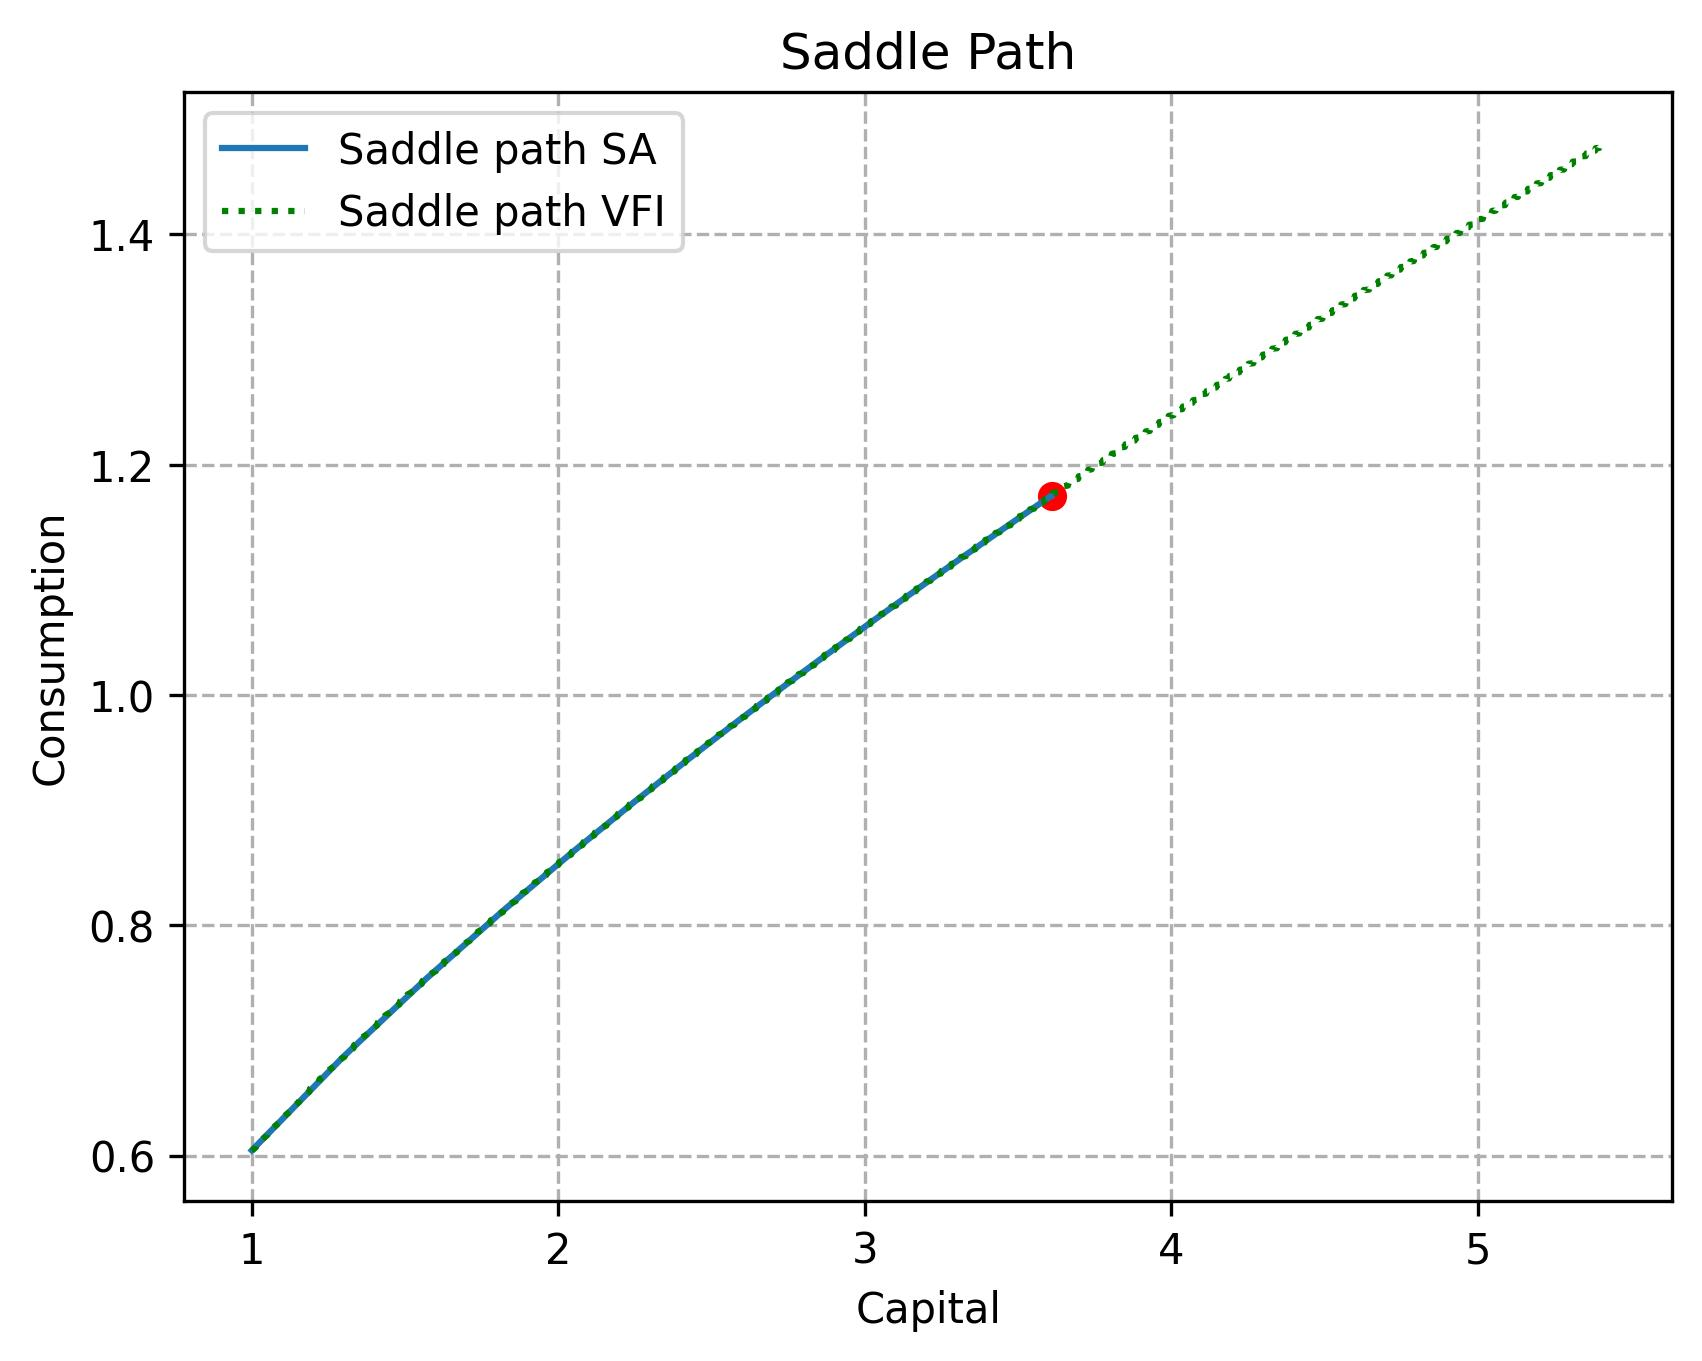
\includegraphics[width=0.8\textwidth]{pic.jpg} % Укажите имя вашего файла
    \caption{Решение методом VFI} % Подпись под картинкой
    \label{fig:my_image} % Метка для ссылок
\end{figure}
} % для размера текста , в самом начале дока поставил: {\fontsize{14pt}{20pt}\selectfont  
\end{document}

